\documentclass[12pt,a4paper,oneside]{book}

\usepackage[utf-8]{inputenc}
\usepackage[romanian]{babel}
\usepackage[margin=2cm]{geometry}
\usepackage{graphicx}
\usepackage{xcolor}
\usepackage{listings}
\usepackage{hyperref}
\usepackage{fancyhdr}
\usepackage{amsmath}
\usepackage{amssymb}
\usepackage{tikz}
\usepackage{pgfplots}
\usepackage{float}
\usepackage{array}
\usepackage{booktabs}
\usepackage{tabularx}
\usepackage{tcolorbox}
\usepackage{mdframed}

% ========== Configurare stil cod ==========
\lstset{
    language=C,
    basicstyle=\ttfamily\small,
    keywordstyle=\color{blue}\bfseries,
    commentstyle=\color{gray}\itshape,
    stringstyle=\color{red},
    breaklines=true,
    showstringspaces=false,
    tabsize=4,
    frame=single,
    framerule=0.5pt,
    backgroundcolor=\color{lightgray!20}
}

% ========== Configurare culori ==========
\definecolor{darkblue}{rgb}{0,0,0.5}
\definecolor{lightblue}{rgb}{0.8,0.9,1}
\definecolor{darkgreen}{rgb}{0,0.5,0}
\definecolor{lightgreen}{rgb}{0.8,1,0.8}

% ========== Antet și subsol ==========
\pagestyle{fancy}
\fancyhf{}
\fancyhead[L]{\textit{PCD T31 - Audio Analysis SOAP Server}}
\fancyhead[R]{\thepage}
\fancyfoot[C]{\small Documentație tehnică - 2024}

% ========== Comenzi personalizate ==========
\newcommand{\conceptbox}[2]{
\begin{tcolorbox}[colback=lightblue,colframe=darkblue,title=#1]
#2
\end{tcolorbox}
}

\newcommand{\warningbox}[1]{
\begin{tcolorbox}[colback=yellow!10,colframe=orange,title=\textbf{Atenție}]
#1
\end{tcolorbox}
}

\newcommand{\codefile}[2]{
\subsection*{Fișier: \texttt{#1}}
}

% ========== DOCUMENT START ==========
\title{
    \textbf{PCD T31 - Audio Analysis SOAP Server}\\
    \vspace{0.5cm}
    \large Documentație Tehnică Detaliată
}
\author{Sistem de Procesare Distribuită a Spectrogramelor Audio}
\date{\today}

\begin{document}

\maketitle

\tableofcontents
\newpage

% ========== CAPITOL 1 ==========
\chapter{Introducere și Descriere Generală}

\section{Ce este PCD T31?}

\textbf{PCD T31} (Proiect de Calcul Distribuit T31) este un sistem distribuit specializat în \textbf{analiza și procesarea spectrogramelor audio} utilizând o arhitectură client-server bazată pe web services SOAP. Sistemul este designed pentru a procesa fișiere audio (WAV, MP3, etc.) și a genera reprezentări spectrogram (Mel-spectrograme) care sunt utile în aplicații precum:

\begin{itemize}
    \item \textbf{Recunoașterea vorbirii} - extragerea caracteristicilor audio
    \item \textbf{Clasificare muzică} - identificarea genurilor muzicale
    \item \textbf{Detecție sunete} - identificarea evenimentelor audio
    \item \textbf{Procesare semnal} - analiza frecvență-timp a semnalelor
\end{itemize}

\section{Caracteristicile Principale}

Sistemul PCD T31 oferă următoarele funcționalități:

\begin{table}[H]
\centering
\begin{tabularx}{\textwidth}{|l|X|}
\hline
\textbf{Caracteristică} & \textbf{Descriere} \\
\hline
\textbf{Arhitectură Client-Server} & Model standard de comunicare cu SOAP web services \\
\hline
\textbf{Procesare Distribuită} & Utilizează \texttt{fork()} pentru izolarea computațiilor în procese separate \\
\hline
\textbf{Prelucrare Audio} & Încarcă și resamplează fișiere audio folosind LibrosaC \\
\hline
\textbf{Generare Mel-Spectrograme} & Calculează reprezentări timp-frecvență cu banduri Mel \\
\hline
\textbf{Configurare Dinamică} & Setări runtime via fișiere libconfig \\
\hline
\textbf{Operații Sigure POSIX} & Folosește syscall-uri POSIX direct (write, read) \\
\hline
\textbf{Gestionare Multiprocese} & Suport pentru handlere concurenți prin forking \\
\hline
\end{tabularx}
\caption{Caracteristici principale ale sistemului PCD T31}
\end{table}

\section{Componente Majore}

Sistemul constă din următoarele componente principale:

\begin{enumerate}
    \item \textbf{Server SOAP} (\texttt{serverds}) - Endpoint central de procesare
    \item \textbf{Client SOAP} (\texttt{inetclient}) - Aplicație client pentru conectare
    \item \textbf{Modul Procesare} (\texttt{processing}) - Logică de calcul audio
    \item \textbf{Loader Configurație} (\texttt{config\_loader}) - Citire setări
    \item \textbf{Interfață SOAP} (gSOAP) - Comunicare web services
\end{enumerate}

\newpage

% ========== CAPITOL 2 ==========
\chapter{Arhitectură și Design}

\section{Model de Arhitectură}

\subsection{Diagramă Arhitecturii}

\begin{center}
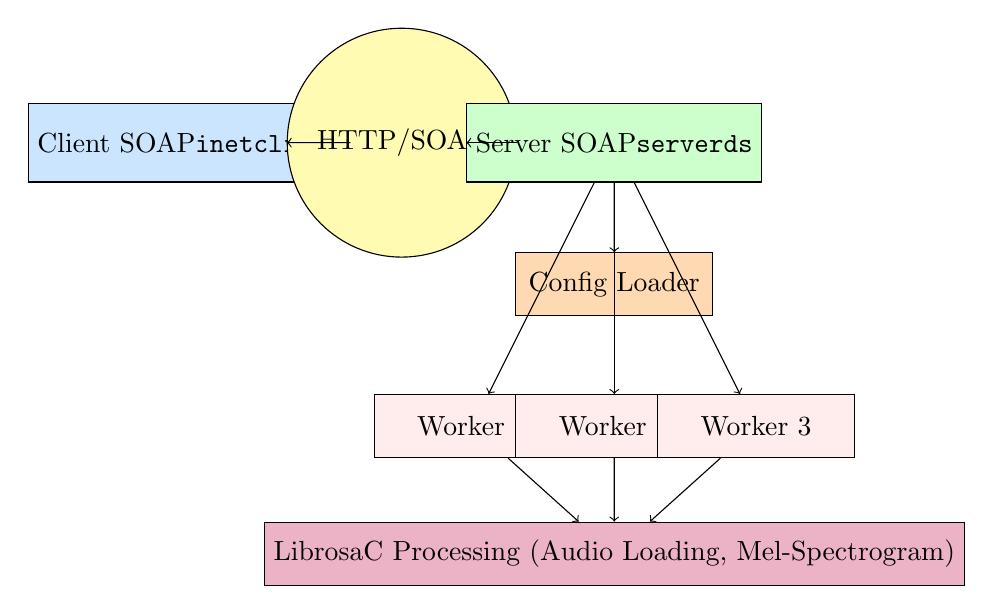
\begin{tikzpicture}[scale=0.9]
    % Client
    \node[draw, rectangle, fill=lightblue, minimum width=3cm, minimum height=1cm] (client) at (1, 6) 
        {Client SOAP \\ \texttt{inetclient}};
    
    % Network
    \node[draw, circle, fill=yellow!30, inner sep=0.3cm] (network) at (4, 6) {HTTP/SOAP};
    
    % Server principal
    \node[draw, rectangle, fill=lightgreen, minimum width=3cm, minimum height=1cm] (server) at (7, 6) 
        {Server SOAP \\ \texttt{serverds}};
    
    % Config loader
    \node[draw, rectangle, fill=orange!30, minimum width=2.5cm, minimum height=0.8cm] (config) at (7, 4) 
        {Config Loader};
    
    % Fork processes
    \node[draw, rectangle, fill=pink!30, minimum width=2.5cm, minimum height=0.8cm] (fork1) at (5, 2) 
        {Worker 1};
    \node[draw, rectangle, fill=pink!30, minimum width=2.5cm, minimum height=0.8cm] (fork2) at (7, 2) 
        {Worker 2};
    \node[draw, rectangle, fill=pink!30, minimum width=2.5cm, minimum height=0.8cm] (fork3) at (9, 2) 
        {Worker 3};
    
    % Processing
    \node[draw, rectangle, fill=purple!30, minimum width=7cm, minimum height=0.8cm] (processing) at (7, 0.2) 
        {LibrosaC Processing (Audio Loading, Mel-Spectrogram)};
    
    % Arrows
    \draw[->] (client) -- (network);
    \draw[->] (network) -- (server);
    \draw[->] (server) -- (config);
    \draw[->] (server) -- (fork1);
    \draw[->] (server) -- (fork2);
    \draw[->] (server) -- (fork3);
    \draw[->] (fork1) -- (processing);
    \draw[->] (fork2) -- (processing);
    \draw[->] (fork3) -- (processing);
    
\end{tikzpicture}
\end{center}

\subsection{Fluxul de Comunicare}

Comunicarea dintre client și server urmează următorii pași:

\begin{enumerate}
    \item \textbf{Inițializare Client}: Clientul se conectează la endpoint-ul SOAP al serverului
    \item \textbf{Construire Request}: Se creează structura \texttt{AnalyzeAudioRequest} cu parametrii (fișier, SR, Mel bands)
    \item \textbf{Trimitere SOAP}: Se apelează \texttt{soap\_call\_ns\_\_analyzeAudio()}
    \item \textbf{Accept Server}: Serverul acceptă conexiunea și forkează un worker
    \item \textbf{Procesare}: Workerul execută \texttt{process\_spectrogram()}
    \item \textbf{Răspuns**: Se returnează metadate (durată, sample rate, cale output)
    \item \textbf{Cleanup}: Procesele worker se termină, client primește răspunsul
\end{enumerate}

\section{Principiile de Design}

\subsection{Izolarea prin Fork()}

\conceptbox{Principiul Izolării}{
Fiecare request SOAP este procesat în procesul \textbf{copil} generat prin \texttt{fork()}. Aceasta oferă:
\begin{itemize}
    \item \textbf{Protecție}: Crash-ul LibrosaC nu afectează serverul principal
    \item \textbf{Concurență}: Multiplii clienți sunt serviți în paralel
    \item \textbf{Curățare}: La ieșire, memoria procesului copil se eliberează automat
\end{itemize}
}

\subsection{Operații Sigure POSIX}

Codul folosește \textbf{apeluri de sistem POSIX} direct în loc de buffering-ul C standard:

\begin{lstlisting}
/* Sigur - async-signal-safe */
write(STDERR_FILENO, msg, sizeof(msg) - 1);

/* NESIGUR în signal handlers */
/* printf("...");  DANGER! */
\end{lstlisting}

\warningbox{
Funcțiile C standard (\texttt{printf}, \texttt{fwrite}) \textbf{NU} sunt signal-safe. În handlere de semnal, trebuie folosite direct syscall-urile POSIX!
}

\section{Ciclu de Viață al unui Request}

\begin{figure}[H]
\centering
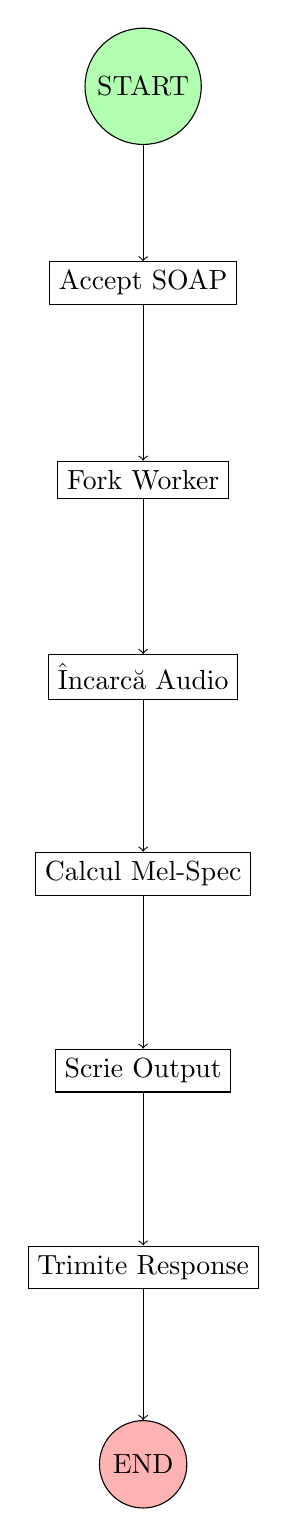
\begin{tikzpicture}[node distance=2.5cm]
    \node (start) [draw, circle, fill=green!30] {START};
    \node (accept) [draw, rectangle, below of=start] {Accept SOAP};
    \node (fork) [draw, rectangle, below of=accept] {Fork Worker};
    \node (load) [draw, rectangle, below of=fork] {Încarcă Audio};
    \node (mel) [draw, rectangle, below of=load] {Calcul Mel-Spec};
    \node (write) [draw, rectangle, below of=mel] {Scrie Output};
    \node (response) [draw, rectangle, below of=write] {Trimite Response};
    \node (end) [draw, circle, fill=red!30, below of=response] {END};
    
    \draw[->] (start) -- (accept);
    \draw[->] (accept) -- (fork);
    \draw[->] (fork) -- (load);
    \draw[->] (load) -- (mel);
    \draw[->] (mel) -- (write);
    \draw[->] (write) -- (response);
    \draw[->] (response) -- (end);
\end{tikzpicture}
\caption{Ciclu de viață al unui request SOAP}
\end{figure}

\newpage

% ========== CAPITOL 3 ==========
\chapter{Componente Tehnice Detaliate}

\section{Server SOAP}

\subsection{Descriere Generală}

Serverul \texttt{serverds} este nucleul sistemului. El:
\begin{itemize}
    \item Ascultă pe un port TCP (default: 8080)
    \item Acceptă conexiuni SOAP și distribuie request-urile
    \item Gestionează procesele copil și semnalele
    \item Citește configurația la pornire
\end{itemize}

\subsection{Structuri de Date}

\begin{lstlisting}
typedef struct {
    int  port;                           /* Port SOAP */
    int  max_workers;                    /* Max procese concurrent */
    int  log_level;                      /* Nivelul logging */
    char output_dir[MAX_PATH_LEN];       /* Directorul output */
    char soap_endpoint[MAX_PATH_LEN];    /* URL endpoint SOAP */
} server_config_t;
\end{lstlisting}

Această structură conține \textbf{configurația runtime} citită din fișierul de configurație \texttt{server.cfg}.

\subsection{Fluxul Principal al Serverului}

\begin{lstlisting}[caption=Fluxul principal de execuție]
/* 1. Inițializare */
config_load(cfg_path, &g_cfg);
server_config_t g_cfg;

/* 2. Creare socket SOAP */
master = soap_bind(soap, NULL, cfg->port, SOAP_BACKLOG);

/* 3. Ciclu de acceptare (în thread principal) */
while (g_running) {
    slave = soap_accept(soap);
    pid = fork();
    
    if (pid == 0) {
        /* Proces copil - serveșă request */
        soap_serve(soap);
        exit(EXIT_SUCCESS);
    }
    
    /* Proces părinte - reapă zombii */
    while (waitpid(-1, NULL, WNOHANG) > 0);
}
\end{lstlisting}

\subsection{Gestionarea Semnalelor}

Serverul instalează un handler pentru \texttt{SIGTERM} care activează graceful shutdown:

\begin{lstlisting}
static void sigterm_handler(int sig) {
    g_running = 0;
    /* write() este async-signal-safe */
    write(STDERR_FILENO, msg, sizeof(msg) - 1);
}

signal(SIGTERM, sigterm_handler);
\end{lstlisting}

La primirea semnalului, serverul:
1. Setează \texttt{g\_running = 0}
2. Iese din ciclu
3. Așteaptă toți copiii cu \texttt{wait()}

\section{Client SOAP}

\subsection{Descriere Generală}

Clientul \texttt{inetclient} este aplicația care inițiază request-urile către server. Oferă:
\begin{itemize}
    \item Parsearea argumentelor din linia de comandă
    \item Citire din variabile de mediu (PCD\_SERVER)
    \item Construire request SOAP cu parametrii audio
    \item Recepție și procesare răspunsuri
\end{itemize}

\subsection{Opțiuni de Linie de Comandă}

\begin{table}[H]
\centering
\begin{tabularx}{\textwidth}{|l|l|X|}
\hline
\textbf{Opțiune} & \textbf{Argument} & \textbf{Descriere} \\
\hline
\texttt{-s} & URL & URL endpoint SOAP (default: \texttt{http://localhost:8080/soap}) \\
\hline
\texttt{-f} & FILE & Cale la fișierul audio (obligatoriu) \\
\hline
\texttt{-m} & MELS & Numărul de benzi Mel (default: 128) \\
\hline
\texttt{-r} & SR & Sample rate țintă în Hz (default: 22050) \\
\hline
\texttt{-h} & - & Afișează ajutorul \\
\hline
\end{tabularx}
\caption{Opțiuni client SOAP}
\end{table}

\subsection{Variabile de Mediu}

\begin{lstlisting}
# Suprascrie serverul implicit
export PCD_SERVER="http://myserver:9090/soap"
./inetclient -f audio.wav
\end{lstlisting}

\subsection{Exemplu de Utilizare}

\begin{lstlisting}
# Utilizare simplă
./inetclient -f music.wav

# Utilizare avansată cu parametrii custom
./inetclient -s http://server.example.com:9090/soap \
             -f audio.mp3 \
             -m 256 \
             -r 16000

# Utilizare cu variabilă de mediu
PCD_SERVER="http://192.168.1.100:8080/soap" \
./inetclient -f song.wav -m 64
\end{lstlisting}

\section{Modul Procesare}

\subsection{Descriere Generală}

Modulul \texttt{processing} conține logica de calcul DSP pentru generarea spectrogramelor. Folosește \textbf{LibrosaC}, o bibliotecă C care oferă bindings pentru funcționalitățile Python librosa.

\subsection{Structuri de Date}

\begin{lstlisting}
/* Request-ul de procesare */
typedef struct {
    char input_path[MAX_PATH_LEN];   /* Cale fișier audio */
    char output_path[MAX_PATH_LEN];  /* Cale fișier output */
    int  target_sr;                  /* Sample rate țintă */
    int  n_fft;                      /* FFT size */
    int  hop_length;                 /* Hop length (overlap) */
    int  n_mels;                     /* Benzi Mel */
} proc_request_t;

/* Rezultatul procesării */
typedef struct {
    int    status;                   /* Status code */
    char   error_msg[256];           /* Mesaj eroare */
    char   output_path[MAX_PATH_LEN];/* Cale rezultat */
    int    sample_rate;              /* SR efectiv */
    int    n_samples;                /* Numărul de sample */
    double duration_s;               /* Durată în secunde */
    int    n_mels;                   /* Benzi Mel generate */
    int    n_frames;                 /* Frames de spectrogram */
} proc_result_t;
\end{lstlisting}

\subsection{Etapele Procesării}

Procesarea audio urmează următorii pași:

\begin{enumerate}
    \item \textbf{Încarcă audio} - \texttt{librosa\_load()}: Decodează fișier, resamplează
    \item \textbf{Generează Mel-spectrogram} - \texttt{librosa\_melspectrogram()}
    \item \textbf{Conversie în dB} - \texttt{librosa\_amplitude\_to\_db()}
    \item \textbf{Scrie output} - Salvează binarul în fișier
    \item \textbf{Returnează metadate} - Durată, sample rate, frames
\end{enumerate}

\subsection{Algoritmi de Procesare}

\subsubsection{Încărcarea și Resamplarea Audio}

\begin{lstlisting}
int librosa_load(const char *path,
                 int target_sr,      /* Sample rate țintă */
                 int mono,           /* 1 = mono, 0 = stereo */
                 float **samples,    /* Buffer output */
                 int *n_samples,     /* Count output */
                 int *sample_rate);  /* SR efectiv */
\end{lstlisting}

\textbf{Explicație}: Funcția citește un fișier audio (WAV, MP3, etc.), îl convertește la mono (dacă necesar), îl resamplează la \texttt{target\_sr} și returnează buffer-ul de float-uri.

\subsubsection{Generarea Mel-Spectrogram}

\begin{lstlisting}
int librosa_melspectrogram(const float *samples,
                           int n_samples,
                           int sample_rate,
                           int n_fft,          /* FFT size (ex: 2048) */
                           int hop_length,     /* Overlap (ex: 512) */
                           int n_mels,         /* Benzi (ex: 128) */
                           float **mel_spec,   /* Output matrix */
                           int *out_n_mels,
                           int *out_n_frames);
\end{lstlisting}

\warningbox{
\textbf{Parametrii importanți}:
\begin{itemize}
    \item \textbf{n\_fft}: Dimensiunea transformatei Fourier. Valori mai mari = rezoluție frecvență mai bună
    \item \textbf{hop\_length}: Hop-ul între frame-uri. Valori mai mici = rezoluție timp mai bună
    \item \textbf{n\_mels}: Numărul de benzi Mel. 128 este standard pentru vorbire, 256 pentru muzică
\end{itemize}
}

\subsubsection{Conceptul de Mel-Spectrogram}

\begin{tcolorbox}[colback=lightblue,colframe=darkblue,title=Ce este o Mel-Spectrogram?]
O Mel-spectrogram este o reprezentare a semnalului audio în timp-frecvență, unde:
\begin{itemize}
    \item \textbf{Axa X}: Timp (secunde)
    \item \textbf{Axa Y}: Frecvență în scală Mel (asemănătoare percepției umane)
    \item \textbf{Intensitate (culoare)}: Energie spectrale (putere)
\end{itemize}

Formula conversiei Hz → Mel:
$$m = 2595 \log_{10}\left(1 + \frac{f}{700}\right)$$

Melele sunt benzi de frecvență care imitează modul în care urechea umană percepe frecvențele. Sunt mai dense la frecvențe joase și mai rare la frecvențe înalte.
\end{tcolorbox}

\section{Config Loader}

\subsection{Descriere Generală}

Modulul \texttt{config\_loader} încarcă setările serverului dintr-un fișier de configurație \textbf{libconfig} (format text ușor de citit).

\subsection{Fișier de Configurație}

\begin{lstlisting}[caption=Exemplu server.cfg]
server:
{
    port = 8080;
    max_workers = 4;
    output_dir = "./output";
    soap_endpoint = "http://localhost:8080/soap";
    log_level = 1;
};

processing:
{
    default_sample_rate = 22050;
    default_n_fft       = 2048;
    default_hop_length  = 512;
    default_n_mels      = 128;
};
\end{lstlisting}

\subsection{Funcții Publice}

\begin{lstlisting}
/* Încarcă configurația dintr-un fișier */
int config_load(const char *path, server_config_t *out);

/* Eliberează resursele configurației */
void config_free(server_config_t *cfg);
\end{lstlisting}

\section{Interfața SOAP}

\subsection{Ce este SOAP?}

\conceptbox{SOAP - Simple Object Access Protocol}{
SOAP este un protocol XML pentru schimbul de mesaje între aplicații. Beneficii:
\begin{itemize}
    \item Platform-independent
    \item Limbaj-agnostic
    \item Ușor de debugat (mesajele sunt text XML)
    \item Suport nativ pentru web services
\end{itemize}
}

\subsection{gSOAP}

\textbf{gSOAP} este o bibliotecă C/C++ care simplifică crearea de server SOAP. Din definiții de tip C, generează:
\begin{itemize}
    \item \texttt{soapC.c} - Serializare/deserializare
    \item \texttt{soapServer.c} - Dispatcher server
    \item \texttt{soapClient.c} - Proxy client
    \item \texttt{soapH.h} - Structuri și funcții
\end{itemize}

\subsection{Definiția Serviciilor SOAP}

\begin{lstlisting}[caption=Exemplu WSDL/IDL gSOAP]
/* Namespace */
//gsoap ns schema namespace: http://example.com/pcd

struct ns__AnalyzeAudioRequest {
    char *inputFilePath;
    int targetSampleRate;
    int nMels;
    int nFft;
    int hopLength;
};

struct ns__AnalyzeAudioResponse {
    int status;
    char *errorMsg;
    char *outputPath;
    int sampleRate;
    int nSamples;
    double durationSeconds;
};

/* Definiția serviciului */
int ns__analyzeAudio(
    struct ns__AnalyzeAudioRequest *req,
    struct ns__AnalyzeAudioResponse *res
);
\end{lstlisting}

\newpage

% ========== CAPITOL 4 ==========
\chapter{Flux de Date și Comunicare}

\section{Diagrama Flux de Date}

\begin{center}
\begin{tikzpicture}[scale=0.85]
    % Client
    \node[draw, rectangle, fill=lightblue, minimum width=3cm] (c1) at (1, 8) {Client};
    
    % SOAP HTTP
    \node[draw, ellipse, fill=yellow!30] (soap1) at (4, 8) {HTTP POST};
    \node[draw, rectangle, minimum width=2cm] (soap_msg1) at (4, 7) {\texttt{<soap:Envelope>}};
    
    % Server listen
    \node[draw, rectangle, fill=lightgreen, minimum width=3cm] (s1) at (7, 8) {Server Port 8080};
    \node[draw, rectangle, minimum width=3cm] (s2) at (7, 6.5) {Parse SOAP};
    
    % Fork
    \node[draw, rectangle, fill=pink!30, minimum width=3cm] (fork) at (7, 5) {fork() Worker};
    
    % Processing
    \node[draw, rectangle, fill=purple!30, minimum width=3cm] (proc1) at (7, 3.5) {librosa\_load()};
    \node[draw, rectangle, fill=purple!30, minimum width=3cm] (proc2) at (7, 2.5) {librosa\_melspectrogram()};
    \node[draw, rectangle, fill=purple!30, minimum width=3cm] (proc3) at (7, 1.5) {write() output};
    
    % Response
    \node[draw, ellipse, fill=yellow!30] (soap2) at (4, 3) {HTTP Response};
    \node[draw, rectangle, minimum width=2cm] (soap_msg2) at (4, 2) {\texttt{<soap:Envelope>}};
    
    % Client receive
    \node[draw, rectangle, fill=lightblue, minimum width=3cm] (c2) at (1, 2) {Client recv()};
    
    % Arrows
    \draw[->] (c1) -- (soap1);
    \draw[->] (soap1) -- (s1);
    \draw[->] (s1) -- (s2);
    \draw[->] (s2) -- (fork);
    \draw[->] (fork) -- (proc1);
    \draw[->] (proc1) -- (proc2);
    \draw[->] (proc2) -- (proc3);
    \draw[->] (proc3) -- (soap2);
    \draw[->] (soap2) -- (c2);
    
\end{tikzpicture}
\end{center}

\section{Format Mesaj SOAP}

\subsection{Request}

\begin{lstlisting}[language=xml,caption=Exemplu SOAP Request]
<?xml version="1.0" encoding="UTF-8"?>
<SOAP-ENV:Envelope
  xmlns:SOAP-ENV="http://schemas.xmlsoap.org/soap/envelope/"
  xmlns:ns="http://example.com/pcd">
  <SOAP-ENV:Body>
    <ns:analyzeAudio>
      <inputFilePath>/path/to/audio.wav</inputFilePath>
      <targetSampleRate>22050</targetSampleRate>
      <nMels>128</nMels>
      <nFft>2048</nFft>
      <hopLength>512</hopLength>
    </ns:analyzeAudio>
  </SOAP-ENV:Body>
</SOAP-ENV:Envelope>
\end{lstlisting}

\subsection{Response}

\begin{lstlisting}[language=xml,caption=Exemplu SOAP Response]
<?xml version="1.0" encoding="UTF-8"?>
<SOAP-ENV:Envelope
  xmlns:SOAP-ENV="http://schemas.xmlsoap.org/soap/envelope/"
  xmlns:ns="http://example.com/pcd">
  <SOAP-ENV:Body>
    <ns:analyzeAudioResponse>
      <status>0</status>
      <errorMsg></errorMsg>
      <outputPath>/output/spectrogram_12345.bin</outputPath>
      <sampleRate>22050</sampleRate>
      <nSamples>441000</nSamples>
      <durationSeconds>20.0</durationSeconds>
      <nMels>128</nMels>
      <nFrames>1293</nFrames>
    </ns:analyzeAudioResponse>
  </SOAP-ENV:Body>
</SOAP-ENV:Envelope>
\end{lstlisting}

\section{Structuri de Date în Comunicare}

\subsection{Request Structure}

\begin{table}[H]
\centering
\begin{tabularx}{\textwidth}{|l|l|X|}
\hline
\textbf{Câmp} & \textbf{Tip} & \textbf{Descriere} \\
\hline
\texttt{inputFilePath} & string & Cale absolută/relativă la fișierul audio \\
\hline
\texttt{targetSampleRate} & int & Hz la care se resamplează (ex: 22050) \\
\hline
\texttt{nMels} & int & Benzi Mel (ex: 128, 256) \\
\hline
\texttt{nFft} & int & Dimensiune FFT (ex: 2048, 4096) \\
\hline
\texttt{hopLength} & int & Hop-ul între frame-uri (ex: 512) \\
\hline
\end{tabularx}
\caption{Câmpurile request SOAP}
\end{table}

\subsection{Response Structure}

\begin{table}[H]
\centering
\begin{tabularx}{\textwidth}{|l|l|X|}
\hline
\textbf{Câmp} & \textbf{Tip} & \textbf{Descriere} \\
\hline
\texttt{status} & int & 0 = succes, <0 = eroare \\
\hline
\texttt{errorMsg} & string & Mesaj de eroare (dacă status < 0) \\
\hline
\texttt{outputPath} & string & Cale la fișierul spectrogram generat \\
\hline
\texttt{sampleRate} & int & Sample rate efectiv după resamplare \\
\hline
\texttt{nSamples} & int & Numărul total de sample în audio \\
\hline
\texttt{durationSeconds} & double & Durată audio în secunde \\
\hline
\texttt{nMels} & int & Benzi Mel generate efectiv \\
\hline
\texttt{nFrames} & int & Numărul de frame-uri în spectrogram \\
\hline
\end{tabularx}
\caption{Câmpurile response SOAP}
\end{table}

\newpage

% ========== CAPITOL 5 ==========
\chapter{Fluxuri de Execuție Detailate}

\section{Fluxul Serverului (serverds)}

\subsection{Inițializare}

\begin{lstlisting}[caption=Inițializare server]
int main(int argc, char *argv[]) {
    /* 1. Parsare argumente */
    const char *cfg_path = DEFAULT_CONFIG_PATH;
    int port_override = 0;
    while ((opt = getopt(argc, argv, "c:p:vh")) != -1) {
        switch (opt) {
            case 'c': cfg_path = optarg; break;
            case 'p': port_override = atoi(optarg); break;
            /* ... */
        }
    }
    
    /* 2. Încarcă configurație */
    config_load(cfg_path, &g_cfg);
    
    if (port_override > 0)
        g_cfg.port = port_override;
    
    /* 3. Instalează handler SIGTERM */
    signal(SIGTERM, sigterm_handler);
    
    /* 4. Inițializează SOAP runtime */
    struct soap soap;
    soap_init(&soap);
    
    /* 5. Rulează server */
    run_soap_server(&soap, &g_cfg);
    
    return 0;
}
\end{lstlisting}

\subsection{Ciclu Principal}

\begin{lstlisting}[caption=Ciclu principal de acceptare]
while (g_running) {
    /* Acceptă conexiune */
    SOAP_SOCKET slave = soap_accept(soap);
    if (!soap_valid_socket(slave)) {
        if (errno == EINTR) 
            continue;  /* Întrerupt de semnal */
        break;
    }
    
    /* Fork worker */
    pid_t pid = fork();
    
    if (pid < 0) {
        perror("[server] fork");
        continue;
    }
    
    if (pid == 0) {
        /* PROCES COPIL - serveșă request */
        soap_serve(soap);           /* Dispatcher SOAP */
        soap_destroy(soap);
        soap_end(soap);
        soap_done(soap);
        exit(EXIT_SUCCESS);
    }
    
    /* PROCES PĂRINTE - reapă zombii */
    soap_closesock(soap);
    while (waitpid(-1, NULL, WNOHANG) > 0)
        ;  /* Non-blocking reap */
}

/* Așteptă toți copiii finali */
while (wait(NULL) > 0)
    ;
\end{lstlisting}

\subsection{Handler SIGTERM}

\begin{lstlisting}[caption=Handler pentru shutdown]
static volatile sig_atomic_t g_running = 1;

static void sigterm_handler(int sig) {
    (void)sig;  /* Evită warning "unused parameter" */
    
    /* SIGUR: write() este async-signal-safe */
    g_running = 0;
    const char msg[] = "\n[server] Shutting down...\n";
    write(STDERR_FILENO, msg, sizeof(msg) - 1);
    
    /* NESIGUR:
       printf(...);     // DANGER!
       exit(0);         // DANGER!
    */
}
\end{lstlisting}

\section{Fluxul Clientului (inetclient)}

\subsection{Inițializare și Construire Request}

\begin{lstlisting}[caption=Inițializare client SOAP]
int main(int argc, char *argv[]) {
    /* Citire variabilă mediu PCD_SERVER */
    const char *env_server = getenv("PCD_SERVER");
    const char *endpoint = env_server ? 
                          env_server : 
                          DEFAULT_ENDPOINT;
    
    const char *file_path = NULL;
    int n_mels = 128;
    int sample_rate = 22050;
    
    /* Parsare argumente */
    int opt;
    while ((opt = getopt(argc, argv, "s:f:m:r:h")) != -1) {
        switch (opt) {
            case 's': endpoint = optarg; break;
            case 'f': file_path = optarg; break;
            case 'm': n_mels = atoi(optarg); break;
            case 'r': sample_rate = atoi(optarg); break;
            case 'h': print_usage(argv[0]); return 0;
            default: return 1;
        }
    }
    
    if (!file_path) {
        fprintf(stderr, "[client] Error: -f <file> required\n");
        return 1;
    }
    
    /* Construire request */
    struct ns__AnalyzeAudioRequest req;
    struct ns__AnalyzeAudioResponse res;
    
    memset(&req, 0, sizeof(req));
    memset(&res, 0, sizeof(res));
    
    req.inputFilePath = (char *)file_path;
    req.targetSampleRate = sample_rate;
    req.nMels = n_mels;
    req.nFft = 2048;
    req.hopLength = 512;
    
    /* Inițializare SOAP runtime */
    struct soap soap;
    soap_init(&soap);
    
    return 0;
}
\end{lstlisting}

\subsection{Apelul SOAP}

\begin{lstlisting}[caption=Executarea apelului SOAP]
/* Apel SOAP */
int rc = soap_call_ns__analyzeAudio(&soap, endpoint, NULL, 
                                     &req, &res);

if (rc != SOAP_OK) {
    /* Eroare SOAP */
    soap_print_fault(&soap, stderr);
} else {
    /* Succes */
    printf("[client] Status     : %d\n", res.status);
    printf("[client] Output     : %s\n", res.outputPath);
    printf("[client] Duration   : %.2f s\n", res.durationSeconds);
    printf("[client] Sample Rate: %d Hz\n", res.sampleRate);
    printf("[client] Mel Bands  : %d\n", res.nMels);
    printf("[client] Frames     : %d\n", res.nFrames);
}

/* Cleanup */
soap_destroy(&soap);
soap_end(&soap);
soap_done(&soap);
\end{lstlisting}

\section{Fluxul Procesării Audio}

\subsection{Funcția de Procesare}

\begin{lstlisting}[caption=Procesare audio în worker]
static int process_spectrogram_worker(
    const proc_request_t *req,
    proc_result_t *res)
{
    /* Step 1: Încarcă audio */
    float *samples = NULL;
    int n_samples = 0;
    int sample_rate = 0;
    
    int rc = librosa_load(
        req->input_path,
        req->target_sr,      /* Resamplare țintă */
        1,                   /* Mono */
        &samples,
        &n_samples,
        &sample_rate);
    
    if (rc != 0 || samples == NULL) {
        snprintf(res->error_msg, sizeof(res->error_msg),
                "librosa_load failed");
        return -1;
    }
    
    res->sample_rate = sample_rate;
    res->n_samples = n_samples;
    res->duration_s = (double)n_samples / sample_rate;
    
    /* Step 2: Generează Mel-spectrogram */
    float *mel_spec = NULL;
    int n_mels = 0;
    int n_frames = 0;
    
    rc = librosa_melspectrogram(
        samples, n_samples, sample_rate,
        req->n_fft,
        req->hop_length,
        req->n_mels,
        &mel_spec, &n_mels, &n_frames);
    
    if (rc != 0 || mel_spec == NULL) {
        snprintf(res->error_msg, sizeof(res->error_msg),
                "librosa_melspectrogram failed");
        goto cleanup;
    }
    
    res->n_mels = n_mels;
    res->n_frames = n_frames;
    
    /* Step 3: Scrie output */
    /* ... */
    
cleanup:
    librosa_free(samples);
    librosa_free(mel_spec);
    return rc;
}
\end{lstlisting}

\newpage

% ========== CAPITOL 6 ==========
\chapter{Build și Compilare}

\section{Sistem Build}

Proiectul utilizează \texttt{GNU Make} pentru orchestrarea compilării.

\subsection{Variabile Makefile}

\begin{lstlisting}[caption=Variabile de compilare]
CC      = gcc                     # Compilator
CFLAGS  = -Wall -Wextra ...       # Warnings strict
CFLAGS  += -std=c11               # Standard C11
CFLAGS  += -D_POSIX_C_SOURCE=200809L  # POSIX APIs

DEBUG ?= 0
ifeq ($(DEBUG),1)
    CFLAGS += -g -O0 -DDEBUG      # Debug build
else
    CFLAGS += -O2 -DNDEBUG        # Release build
endif

# Biblioteci
LIBS_SOAP    = -lgsoap
LIBS_CONFIG  = -lconfig
LIBS_LIBROSA = -lrosacpp
LIBS_THREAD  = -lpthread
LIBS_MATH    = -lm
\end{lstlisting}

\subsection{Compilare}

\begin{lstlisting}[language=bash,caption=Comenzi de compilare]
# Build default (release)
make all

# Build cu debug info
make DEBUG=1

# Build doar server
make serverds

# Build doar client
make inetclient

# Curățare obiecte
make clean

# Rebuild complet
make clean all
\end{lstlisting}

\subsection{Fișiere Generate de gSOAP}

\begin{table}[H]
\centering
\begin{tabularx}{\textwidth}{|l|l|X|}
\hline
\textbf{Fișier} & \textbf{Tip} & \textbf{Descriere} \\
\hline
\texttt{soapC.c} & Source & Serializare/deserializare XML \\
\hline
\texttt{soapServer.c} & Source & Dispatcher server \\
\hline
\texttt{soapClient.c} & Source & Proxy client \\
\hline
\texttt{soapH.h} & Header & Structuri generate \\
\hline
\end{tabularx}
\caption{Fișiere generate de gSOAP}
\end{table}

\section{Dependințe Externe}

\begin{table}[H]
\centering
\begin{tabularx}{\textwidth}{|l|l|X|}
\hline
\textbf{Bibliotecă} & \textbf{Tip} & \textbf{Descriere} \\
\hline
\textbf{gSOAP} & Web Services & Protocol SOAP, gen HTTP \\
\hline
\textbf{libconfig} & Config & Parser configurație \\
\hline
\textbf{LibrosaC} & DSP & Audio processing (C bindings) \\
\hline
\textbf{pthreads} & Threading & POSIX threads \\
\hline
\textbf{libm} & Math & Funcții matematice \\
\hline
\end{tabularx}
\caption{Dependințe externe ale proiectului}
\end{table}

\subsection{Instalare Dependințe}

\begin{lstlisting}[language=bash]
# Ubuntu/Debian
sudo apt-get install libgsoap-dev libconfig-dev libm-dev

# Pentru LibrosaC (build din sursă sau pachet custom)
# See: https://github.com/librosa/librosa-c

# Verificare compilare
gcc --version
make --version
\end{lstlisting}

\newpage

% ========== CAPITOL 7 ==========
\chapter{Managementul Proceselor}

\section{Model de Procesare}

\subsection{Arhitectură Fork-Worker}

PCD T31 folosește modelul \textbf{fork-worker}:

\begin{enumerate}
    \item \textbf{Thread principal} acceptă conexiuni SOAP
    \item \textbf{La fiecare request}, se creează un proces copil via \texttt{fork()}
    \item \textbf{Copilul} execută \texttt{soap\_serve()} și procesează request
    \item \textbf{Copilul} se termină, parent-ul recoltează resurse via \texttt{waitpid()}
\end{enumerate}

\subsection{Avantaje}

\begin{itemize}
    \item \textbf{Izolație}: Crash LibrosaC nu afectează server
    \item \textbf{Concurență}: Multiplii clienți procesați în paralel
    \item \textbf{Simplitate}: Nu necesită threading complex
    \item \textbf{Scalabilitate}: Suportă max\_workers concurrent
\end{itemize}

\section{Gestionarea Zombilor}

\subsection{Problemă: Procese Zombie}

Când un proces copil se termină, părintele trebuie să apeleze \texttt{wait()} sau \texttt{waitpid()} pentru a-i recolta starea. Altfel, copilul rămâne în stare \textbf{zombie} (defunct).

\begin{lstlisting}[caption=Recoltare non-blocking]
/* În ciclu principal */
while (g_running) {
    pid_t slave = soap_accept(soap);
    if (fork() == 0) {
        /* COPIL */
        soap_serve(soap);
        exit(0);
    }
    
    /* PĂRINTE - reapă zombii */
    while (waitpid(-1, NULL, WNOHANG) > 0)
        ;  /* Flag WNOHANG = non-blocking */
}
\end{lstlisting}

\textbf{WNOHANG}: Returnează imediat chiar dacă nu sunt copii zombi. 0 = nicio reacție, > 0 = PID recoltat.

\subsection{Cleanup la Shutdown}

\begin{lstlisting}[caption=Cleanup la terminare server]
/* La primirea SIGTERM */
g_running = 0;  /* Iese din ciclu */

/* Așteptă toți copiii */
while (wait(NULL) > 0)
    ;  /* Fără WNOHANG = blocking */
\end{lstlisting}

\section{Limite de Procese}

\begin{table}[H]
\centering
\begin{tabularx}{\textwidth}{|l|l|X|}
\hline
\textbf{Parametru} & \textbf{Default} & \textbf{Descriere} \\
\hline
\texttt{max\_workers} & 4 & Max procese concurrent (din config) \\
\hline
\texttt{SOAP\_BACKLOG} & 10 & Pending connections în queue \\
\hline
\texttt{SOAP\_TIMEOUT\_S} & 30 & Timeout inactiv (secunde) \\
\hline
\texttt{ulimit -u} & (system) & Max procese per utilizator \\
\hline
\end{tabularx}
\caption{Limite procesare}
\end{table}

\section{Monitorizare Procese}

\subsection{Comenzi Util}

\begin{lstlisting}[language=bash]
# Lista procese server
ps aux | grep serverds

# Monitorizare timp real
top -p $(pgrep serverds)

# Copii ai procesului
pstree -p $(pgrep serverds)

# Statistic resursă
ps aux | grep serverds | awk '{print $6 " KB mem"}'
\end{lstlisting}

\newpage

% ========== CAPITOL 8 ==========
\chapter{Operații POSIX și Siguranță}

\section{De Ce POSIX Syscalls?}

\conceptbox{POSIX vs Standard C}{
\textbf{Standard C (printf, fwrite)}: Bufferate, NU sunt signal-safe.
\\
\textbf{POSIX syscalls (write, read)}: Unbuffered, signal-safe, sigure în handlers.
}

\subsection{Exemplu: Sigterm Handler}

\begin{lstlisting}[caption=Handler SIGTERM cu POSIX]
/* SIGUR - async-signal-safe */
static void sigterm_handler(int sig) {
    g_running = 0;
    write(STDERR_FILENO, msg, len);  /* OK */
}

/* NESIGUR - NU! */
static void bad_handler(int sig) {
    printf("...");      /* DANGER - printf buffering */
    exit(0);            /* DANGER - cleanup nesigur */
    fwrite(...);        /* DANGER - buffered I/O */
}
\end{lstlisting}

\section{Funcții Signal-Safe POSIX}

\begin{table}[H]
\centering
\begin{tabularx}{\textwidth}{|l|l|l|}
\hline
\textbf{Sigur} & \textbf{Nesigur} & \textbf{Categorie} \\
\hline
\texttt{write()} & \texttt{printf()} & I/O \\
\texttt{open()} & \texttt{fopen()} & Fișiere \\
\texttt{close()} & \texttt{fclose()} & Fișiere \\
\texttt{exit()} & (direct cleanup) & Control \\
\texttt{signal()} & (la signal entry) & Semnal \\
\texttt{sleep()} & \texttt{sleep()} & Timp (rar) \\
\hline
\end{tabularx}
\caption{Funcții signal-safe vs unsafe}
\end{table}

\section{File Operations cu Write/Read}

\subsection{Scrierea Buffer Float}

\begin{lstlisting}[caption=Scriere sigură de date float]
static int write_float_array(int fd, const float *data, 
                             size_t n) {
    size_t total = n * sizeof(float);
    const char *ptr = (const char *)data;
    
    while (total > 0) {
        ssize_t written = write(fd, ptr, total);
        if (written < 0) {
            if (errno == EINTR)
                continue;  /* Retry pe semnal */
            return -1;
        }
        ptr += written;
        total -= (size_t)written;
    }
    return 0;  /* Succes */
}
\end{lstlisting}

\textbf{Explicație}:
\begin{itemize}
    \item \texttt{write()} nu garantează scrierea tuturor bytes-ilor deodată
    \item Loop continuă până când sunt scrise toți byte-ii
    \item \texttt{EINTR} înseamnă interrupt de semnal - retry automat
\end{itemize}

\section{Erori Frecvente și Evitare}

\warningbox{
\textbf{Greșeli comune cu syscalls}:
\begin{enumerate}
    \item \textbf{Nu verifi errno} după eșec syscall
    \item \textbf{Nu handlezi EINTR} în loop
    \item \textbf{Nu iei în considerare partial writes} la write()
    \item \textbf{Folosești buffering} în signal handlers
\end{enumerate}
}

\newpage

% ========== CAPITOL 9 ==========
\chapter{Configurație și Personalizare}

\section{Fișierul de Configurație}

\subsection{Locație Default}

Fișierul implicit se găsește la:
\begin{lstlisting}
./config/server.cfg
\end{lstlisting}

Pentru specify alt path:
\begin{lstlisting}[language=bash]
./serverds -c /path/to/custom.cfg
\end{lstlisting}

\subsection{Sintaxă libconfig}

\begin{lstlisting}[caption=Exemplu configurație completă]
# Comentarii cu #

server: {
    # Port TCP pentru SOAP
    port = 8080;
    
    # Max procese worker concurrent
    max_workers = 4;
    
    # Directorul unde se salvează spectrograme
    output_dir = "./output";
    
    # URL endpoint (informativ)
    soap_endpoint = "http://localhost:8080/soap";
    
    # Nivelul logging: 0 = silent, 1 = info, 2 = debug
    log_level = 1;
};

# Setări default procesare (optional)
processing: {
    default_sample_rate = 22050;
    default_n_fft       = 2048;
    default_hop_length  = 512;
    default_n_mels      = 128;
};
\end{lstlisting}

\section{Parametri Configurabili}

\subsection{Port SOAP}

\begin{lstlisting}
# În fișier config
server: { port = 9000; };

# Sau în linia de comandă (suprascrie)
./serverds -p 9000
\end{lstlisting}

\subsection{Directorul Output}

\begin{lstlisting}
server: { output_dir = "/var/pcd-output"; };
\end{lstlisting}

Fișierele spectrogram generate sunt salvate aici sub forma \texttt{spectrogram\_XXXXXXXX.bin}.

\subsection{Parametri Procesare Audio}

\begin{lstlisting}
processing: {
    # Sample rate la care se resamplează audio
    default_sample_rate = 22050;
    
    # Dimensiunea FFT (mai mare = rezoluție frecvență mai bună)
    default_n_fft = 2048;
    
    # Hop-ul dintre frame-uri (mai mic = rezoluție timp mai bună)
    default_hop_length = 512;
    
    # Benzi Mel (128 = vorbire, 256 = muzică)
    default_n_mels = 128;
};
\end{lstlisting}

\warningbox{
\textbf{Trade-off}: FFT mai mare = mai multă computație. Valori comune:
\begin{itemize}
    \item \textbf{Vorbire}: n\_fft=512, hop=160, n\_mels=40-64
    \item \textbf{Muzică}: n\_fft=2048, hop=512, n\_mels=128-256
\end{itemize}
}

\section{Variabile de Mediu}

\subsection{PCD\_SERVER}

Clientul citește \texttt{PCD\_SERVER} pentru URL server implicit:

\begin{lstlisting}[language=bash]
# Override server implicit
export PCD_SERVER="http://192.168.1.100:9000/soap"

# Client folosește URL din mediu
./inetclient -f audio.wav
\end{lstlisting}

\subsection{Alte Variabile Utile}

\begin{table}[H]
\centering
\begin{tabularx}{\textwidth}{|l|X|}
\hline
\textbf{Variabilă} & \textbf{Utilizare} \\
\hline
\texttt{GSOAP\_DEBUG} & Activează debug gSOAP (dacă compilat) \\
\hline
\texttt{LD\_LIBRARY\_PATH} & Path biblioteci dinamice \\
\hline
\end{tabularx}
\caption{Variabile de mediu utile}
\end{table}

\newpage

% ========== CAPITOL 10 ==========
\chapter{Utilizare și Exemplu de Flux}

\section{Start și Stop Server}

\subsection{Start}

\begin{lstlisting}[language=bash]
# Start cu config default (./config/server.cfg)
./serverds

# Start cu config custom
./serverds -c /etc/pcd/config.cfg

# Start pe alt port
./serverds -p 9000

# Start cu verbose
./serverds -v
\end{lstlisting}

\subsection{Output Inițiare}

\begin{lstlisting}
[server] Config loaded from config/server.cfg
[server] Port         : 8080
[server] Workers max  : 4
[server] Output dir   : ./output
[server] Listening on port 8080 (SOAP endpoint: http://localhost:8080/soap)
\end{lstlisting}

\subsection{Stop}

\begin{lstlisting}[language=bash]
# Graceful shutdown (SIGTERM)
kill $(pgrep serverds)

# Force kill (NU recomandat)
kill -9 $(pgrep serverds)
\end{lstlisting}

\section{Exemplu Flux Complet}

\subsection{Pasul 1: Start Server}

\begin{lstlisting}[language=bash]
cd /path/to/pcd-t31
make clean all

# Terminal 1
./serverds -p 8080 -v
# Output: [server] Listening on port 8080 ...
\end{lstlisting}

\subsection{Pasul 2: Pregătire Fișier Audio}

\begin{lstlisting}[language=bash]
# Asigură că ai un fișier audio valid
ls -lh /path/to/audio.wav
\end{lstlisting}

\subsection{Pasul 3: Rulare Client}

\begin{lstlisting}[language=bash]
# Terminal 2 (pe aceeași mașină)
./inetclient -f /path/to/audio.wav

# Output:
# [client] Connecting to: http://localhost:8080/soap
# [client] File         : /path/to/audio.wav
# [client] Mel bands    : 128
# [client] Sample rate  : 22050 Hz
# Status: 0 (succes)
\end{lstlisting}

\subsection{Pasul 4: Verificare Output}

\begin{lstlisting}[language=bash]
ls -lh ./output/
# spectrogram_12345678.bin

# Dimensiune așteptată:
# (n_frames) * (n_mels) * (sizeof(float)) bytes
# Ex: 1293 * 128 * 4 = 661,504 bytes
\end{lstlisting}

\section{Utilizare Avansată}

\subsection{Client Remote}

\begin{lstlisting}[language=bash]
# Server pe alt host
./inetclient -s http://192.168.1.100:8080/soap \
             -f local_audio.wav

# Sau cu variabilă mediu
PCD_SERVER="http://192.168.1.100:8080/soap" \
./inetclient -f local_audio.wav
\end{lstlisting}

\subsection{Parametri Audio Custom}

\begin{lstlisting}[language=bash]
# Mel-spectrogram cu 256 benzi, 16kHz sample rate
./inetclient -f audio.wav \
             -m 256 \
             -r 16000

# Verifică dimensiunea output:
# 256 * (n_frames) * 4 bytes
\end{lstlisting}

\subsection{Batch Processing}

\begin{lstlisting}[language=bash]
#!/bin/bash
for file in *.wav; do
    echo "Processing: $file"
    ./inetclient -f "$file" \
                 -m 128 \
                 -r 22050
    echo "Done: $file"
done
\end{lstlisting}

\section{Troubleshooting}

\subsection{Client nu se conectează}

\begin{lstlisting}[language=bash]
# 1. Verifică dacă serverul rulează
netstat -tuln | grep 8080

# 2. Verifică endpoint-ul
PCD_SERVER="http://localhost:8080/soap" \
./inetclient -f audio.wav

# 3. Verifică firewall
sudo ufw allow 8080
\end{lstlisting}

\subsection{Eroare LibrosaC}

\begin{lstlisting}
[server] librosa_load failed for: /path/to/audio.wav
\end{lstlisting}

Verifică:
\begin{itemize}
    \item Fișierul audio există și este valid
    \item Cale absolută sau relativă corect
    \item Format audio suportat (WAV, MP3, FLAC, etc.)
\end{itemize}

\subsection{Output corect dar goluri}

Spectrograma poate fi nul dacă:
\begin{itemize}
    \item Audio e prea scurt
    \item Sample rate very low
    \item File prea mare (out of memory)
\end{itemize}

\newpage

% ========== CAPITOL 11 ==========
\chapter{Concepte Audio și DSP}

\section{Fundamentele Procesării Audio}

\subsection{Semnal Audio}

Un semnal audio este o succesiune de \textbf{sample-uri} înregistrate la o rată constantă:

$$\text{Semnal} = [s_0, s_1, s_2, \ldots, s_{N-1}]$$

Unde:
\begin{itemize}
    \item $s_i$ este valoarea sample-ului la timp $t_i = i / f_s$
    \item $f_s$ este sample rate (ex: 22050 Hz)
    \item $N$ este numărul total de sample-uri
\end{itemize}

\subsection{Sample Rate și Aliasing}

\conceptbox{Sample Rate și Nyquist}{
Sample rate determină frecvența maximă care poate fi reprezentată:

$$f_{\text{max}} = \frac{f_s}{2}$$

Pentru vorbire: $f_s = 16000$ Hz (frecv max = 8000 Hz).
\\
Pentru muzică: $f_s = 44100$ Hz (frecv max = 22050 Hz).
}

\section{Mel-Spectrogram}

\subsection{De la STFT la Mel}

\subsubsection{Short-Time Fourier Transform (STFT)}

\begin{enumerate}
    \item Împarte semnalul în frame-uri scurte
    \item Aplică fereastră (Hann, Hamming)
    \item Calculează FFT pentru fiecare frame
    \item Rezultat: matrice timp-frecvență cu amplitudini complexe
\end{enumerate}

Dimensiune STFT:
$$\text{(n\_frames, n\_fft/2 + 1)}$$

Unde:
\begin{itemize}
    \item $n\_\text{frames} = \lfloor (N - n\_\text{fft}) / \text{hop\_length} \rfloor + 1$
    \item $n\_\text{fft}$ = dimensiune FFT (ex: 2048)
    \item $\text{hop\_length}$ = hop-ul dintre frame-uri (ex: 512)
\end{itemize}

\subsubsection{Mel-Scale Filterbank}

Se aplică un set de filtre triunghiulare pe scale Mel:

$$\text{Mel}(f) = 2595 \log_{10}\left(1 + \frac{f}{700}\right)$$

Rezultat: matrice $(\text{n\_frames}, \text{n\_mels})$ unde fiecare intrare este energia în banda Mel respectivă.

\subsection{Parametri Importanți}

\begin{table}[H]
\centering
\begin{tabularx}{\textwidth}{|l|l|l|X|}
\hline
\textbf{Parametru} & \textbf{Default} & \textbf{Interval} & \textbf{Efect} \\
\hline
\texttt{n\_fft} & 2048 & 512-4096 & Rezoluție frecvență \\
\hline
\texttt{hop\_length} & 512 & 128-1024 & Rezoluție timp \\
\hline
\texttt{n\_mels} & 128 & 40-256 & Benzi perceptuale \\
\hline
\texttt{f\_min} & 0 & 0+ & Frecvență min (Hz) \\
\hline
\texttt{f\_max} & 22050 & <fs/2 & Frecvență max (Hz) \\
\hline
\end{tabularx}
\caption{Parametri Mel-spectrogram}
\end{table}

\warningbox{
\textbf{Trade-off timp vs frecvență}:
\begin{itemize}
    \item FFT MARE = rezoluție frecvență BUNĂ, rezoluție timp PROASTĂ
    \item FFT MICĂ = rezoluție timp BUNĂ, rezoluție frecvență PROASTĂ
\end{itemize}

Uzual: $\text{hop\_length} \approx n\_\text{fft} / 4$
}

\section{Aplicații Practice}

\subsection{Recunoaștere Vorbire}

\begin{itemize}
    \item Mel-spectrogram intrare la HMM/RNN
    \item n\_mels = 40-64
    \item f\_max = 8000 Hz (nu trebuie frecvențe mai înalte)
    \item Output: text transcription
\end{itemize}

\subsection{Clasificare Muzică}

\begin{itemize}
    \item Mel-spectrogram + CNN
    \item n\_mels = 128-256
    \item Frecvențe pline (0-22050 Hz)
    \item Output: gen muzical (rock, pop, jazz, etc.)
\end{itemize}

\subsection{Detecție Sunete}

\begin{itemize}
    \item Mel-spectrogram + CRNN
    \item n\_mels = 128
    \item Durată segmente: 0.5-2 sec
    \item Output: presence/absence zgomote ambientale
\end{itemize}

\newpage

% ========== CAPITOL 12 ==========
\chapter{Performance și Optimizare}

\section{Analiza Performance}

\subsection{Factori care Afectează Performanța}

\begin{table}[H]
\centering
\begin{tabularx}{\textwidth}{|l|X|X|}
\hline
\textbf{Factor} & \textbf{Impact} & \textbf{Optimizare} \\
\hline
Dimensiune fișier & $\uparrow$ timp procesare & Limita durată input \\
\hline
n\_fft & $\uparrow$ computație FFT & Trade-off rezoluție \\
\hline
hop\_length & $\uparrow$ n\_frames & $\downarrow$ hop\_length \\
\hline
n\_mels & $\uparrow$ filterbank & Valori mici suficiente \\
\hline
Resamplare & Decompresie + resample & Pre-resamplare offline \\
\hline
\end{tabularx}
\caption{Factori de performance}
\end{table}

\subsection{Benchmark}

Timp tipic pe mașină de referință (CPU: Intel i7, RAM: 8GB):

\begin{table}[H]
\centering
\begin{tabularx}{\textwidth}{|l|l|l|}
\hline
\textbf{Durata Audio} & \textbf{Parametri} & \textbf{Timp Procesare} \\
\hline
10 sec & n\_fft=2048, n\_mels=128 & ~0.5 sec \\
\hline
30 sec & n\_fft=2048, n\_mels=128 & ~1.5 sec \\
\hline
60 sec & n\_fft=2048, n\_mels=128 & ~3 sec \\
\hline
300 sec (5 min) & n\_fft=2048, n\_mels=128 & ~15 sec \\
\hline
\end{tabularx}
\caption{Timp procesare tipic}
\end{table}

\section{Optimizări Aplicabile}

\subsection{1. Paralelizare Client}

\begin{lstlisting}[language=bash]
# Procesare paralel multiple fișiere
for file in *.wav; do
    ./inetclient -f "$file" &  # Background
done
wait  # Așteptă toți
\end{lstlisting}

\subsection{2. Caching Output}

Salvează spectrograme generate pentru reuzare:

\begin{lstlisting}
# Script cu caching
CACHE="./cache"
FILE="audio.wav"
HASH=$(md5sum "$FILE" | cut -d' ' -f1)

if [ -f "$CACHE/$HASH.bin" ]; then
    echo "Using cached"
    cp "$CACHE/$HASH.bin" output/
else
    ./inetclient -f "$FILE"
    cp output/*.bin "$CACHE/$HASH.bin"
fi
\end{lstlisting}

\subsection{3. Ajustare Parametri}

\begin{lstlisting}
# Vorbire (mai rapid)
./inetclient -f audio.wav -m 40 -r 16000

# Muzică (mai detaliat dar lent)
./inetclient -f audio.wav -m 256 -r 44100
\end{lstlisting}

\section{Profilare}

\subsection{CPU Profiling}

\begin{lstlisting}[language=bash]
# Compilare cu debug + profiling
make DEBUG=1 PROFILE=1

# Rulare cu gprof
gprof ./serverds gmon.out

# Output: funcții ordonate după CPU time
\end{lstlisting}

\subsection{Memory Profiling}

\begin{lstlisting}[language=bash]
# Valgrind memory check
valgrind --leak-check=full ./serverds

# Output: memory leaks, accesuri greșite
\end{lstlisting}

\newpage

% ========== CAPITOL 13 ==========
\chapter{Concluzie și Resurse}

\section{Rezumat Proiect}

\subsection{Arhitectură Rezumată}

\begin{center}
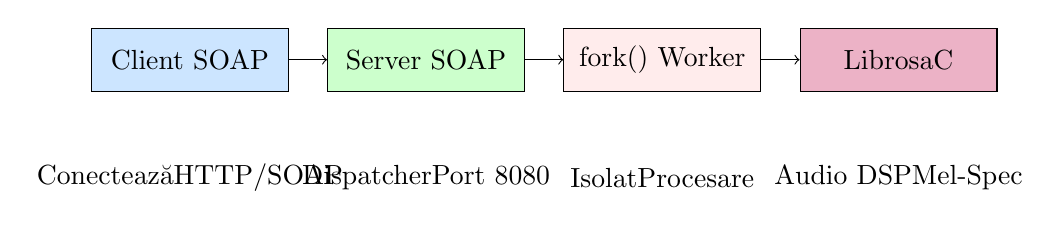
\begin{tikzpicture}[scale=1]
    \node[draw, rectangle, fill=lightblue, minimum width=2.5cm, minimum height=0.8cm] (c) at (0, 2) 
        {Client SOAP};
    \node[draw, rectangle, fill=lightgreen, minimum width=2.5cm, minimum height=0.8cm] (s) at (3, 2) 
        {Server SOAP};
    \node[draw, rectangle, fill=pink!30, minimum width=2.5cm, minimum height=0.8cm] (w) at (6, 2) 
        {fork() Worker};
    \node[draw, rectangle, fill=purple!30, minimum width=2.5cm, minimum height=0.8cm] (l) at (9, 2) 
        {LibrosaC};
    
    \draw[->] (c) -- (s);
    \draw[->] (s) -- (w);
    \draw[->] (w) -- (l);
    
    \node[below of=c, node distance=1.5cm] {Conectează\\HTTP/SOAP};
    \node[below of=s, node distance=1.5cm] {Dispatcher\\Port 8080};
    \node[below of=w, node distance=1.5cm] {Isolat\\Procesare};
    \node[below of=l, node distance=1.5cm] {Audio DSP\\Mel-Spec};
\end{tikzpicture}
\end{center}

\subsection{Chei Conceptuale}

\begin{enumerate}
    \item \textbf{SOAP Web Services}: Protocol standard pentru servicii distribuite
    \item \textbf{Fork-Worker Model}: Izolație și concurență simplistă
    \item \textbf{POSIX Safe Operations}: Syscall-uri sigure în signal handlers
    \item \textbf{Mel-Spectrogram}: Reprezentare timp-frecvență a semnalelor audio
    \item \textbf{libconfig}: Configurație dinamică prin fișiere text
    \item \textbf{LibrosaC}: Bindings C pentru librosa Python
\end{enumerate}

\section{Extensii Posibile}

\subsection{Adăugări de Funcționalități}

\begin{enumerate}
    \item \textbf{Caching Spectrograme}: Evită reprelucrarea aceluiași fișier
    \item \textbf{Batch Processing}: API pentru procesare multiplu fișiere
    \item \textbf{Database Rezultate}: Stocaj metadate în SQL
    \item \textbf{Streaming Audio}: Procesare on-the-fly
    \item \textbf{Transformări Suplimentare}: MFCC, Chroma, Tempogram
    \item \textbf{ML Integration}: Client predicție cu TensorFlow/PyTorch
\end{enumerate}

\subsection{Îmbunătățiri Tehnice}

\begin{enumerate}
    \item \textbf{Thread Pool}: În loc de fork() per request
    \item \textbf{Connection Pooling}: Reuzare conexiuni SOAP
    \item \textbf{Monitoring}: Metrici Prometheus/Grafana
    \item \textbf{Rate Limiting}: Protecție DoS
    \item \textbf{Authentication}: API keys, OAuth
    \item \textbf{Compression}: Transfer date mai mic
\end{enumerate}

\section{Resurse Externe}

\subsection{Documentații și Biblioteci}

\begin{itemize}
    \item \textbf{gSOAP}: \url{https://www.genivia.com/gsoap.html}
    \item \textbf{libconfig}: \url{https://hyperrealm.github.io/libconfig/}
    \item \textbf{LibrosaC}: \url{https://github.com/librosa/librosa-c}
    \item \textbf{POSIX APIs}: \url{https://pubs.opengroup.org/onlinepubs/}
    \item \textbf{Librosa Python}: \url{https://librosa.org/}
\end{itemize}

\subsection{Tutoriale Relevant}

\begin{itemize}
    \item Audio Processing: \url{https://www.coursera.org/learn/audio-signal-processing}
    \item SOAP Web Services: \url{https://www.w3schools.com/xml/xml_soap.asp}
    \item POSIX Programming: \url{https://www.kernel.org/doc/man-pages/}
    \item C Best Practices: \url{https://www.gnu.org/software/libc/manual/}
\end{itemize}

\section{Contacte și Support}

Pentru întrebări sau probleme cu proiectul PCD T31:

\begin{itemize}
    \item \textbf{Documentație}: Consultă \texttt{documentation.tex}
    \item \textbf{Cod}: Comentarii detaliate în fișiere sursă
    \item \textbf{Build}: Verifică \texttt{Makefile}
    \item \textbf{Config}: Editează \texttt{config/server.cfg}
\end{itemize}

\section{Licență și Atribuire}

Proiect PCD T31 - Audio Analysis SOAP Server.

\textit{Documentație tehnică - 2024}

\end{document}
